\chapter{Architecture \& Development}
This chapter will go into detail of the development stages of this project, discussing the various decisions, challenges and problems faced during the development of each individual component in the system, and how they were resolved.

\section{System Overview}
The system is separated into two separate projects, \emph{the web server} which contains the game engine and editor, and \emph{the storage server}. These are both web based applications which host a HTTP server through the Python-based Flask microframework. The overview of the system is shown in Figure \ref, which labels the key components of the system in red.
% Overview of sys arch, diagram to rep the key elements
% Two main separate projects:
% WebServer ---- StorageServer
%	v
% Website
% Editor
% Engine

The majority of the system follows the MVC (Model-View-Controller) software architectural pattern where possible. This pattern simplifies the development of complex systems by separating the data, display and logic sections into more managable subsystems - the model, view and controller respectively. The structure and architectural pattern of each individual component in this system will be described in-depth in Section \ref{section:systemcomponents}.

% ref MVC, simplifies

\section{Development Environment}
The environment used throughout development of the system consisted of the Sublime Text 3 editor running on the Fedora 19 operating system. For each individual Flask project (The web server and storage server) a virtual environment was set up using \textbf{virtualenv}. Use of virtualenv allowed Python 3.4.2 (separate to the version on Fedora 19) and the required Python libraries to be installed individually for each project.

For both projects, Flask and it's dependencies (itsdangerous, Jinja2, MarkupSafe and Werkzeug) were installed using \textbf{pip} in the virtualenv, along with the libraries specific to each project:
\begin{itemize}
	\item Web server:
	\begin{itemize}
		\item Flask-Compress
		\item PyMongo
	\end{itemize}
	\item Storage server:
	\begin{itemize}
		\item GitPython and dependencies (gitdb, smmap)
	\end{itemize}
\end{itemize}

The Git version control system was used to manage the project in this environment, with the project repository being hosted on GitHub as an external backup source. Originally, the two projects were in the same Git repository, however this proved to be unsuitable as rolling back changes on one project could be troublesome. The two projects were split into their own Git repositories using the \textbf{git subtree split} command, which maintained all commit history relevant to each project.

The tools required to manage the Amazon Web Services were also installed in this environment, including the AWS CLI (Command Line Interface), and the Elastic Beanstalk CLI. These tools allow remote management of all AWS resources and quick deployment of applications to the Elastic Beanstalk platform.

\section{System Components}
\label{section:systemcomponents}
	\subsection{Web Server}
	The web server is the core part of the system, where all user requests are handled. Everything the user does on the system goes through the web server, so it must be able to handle a lot of users. For this reason the lightweight `microframework' \emph{Flask} was chosen as the base of the server. %todo more

	\paragraph{Architectural Pattern.}
	The Flask application created for the web server uses a software architectural pattern \emph{similar} to the MVC pattern. Flask lends itself well to the MVC pattern; as each page has it's own route (\textbf{Controller}) and template (\textbf{View}), with the route generally populating the template with data (\textbf{Model}). This can be seen visualised in Figure \ref{fig:flaskprocess} which demonstrates how a request is handled by Flask. A client sends a request to the route, the route then retrieves any requested data (Such as a list of published games), then it renders the template for that route with the data. The generated HTML from the template is sent back as the HTTP response.

	\begin{figure}[h]
		\centering
		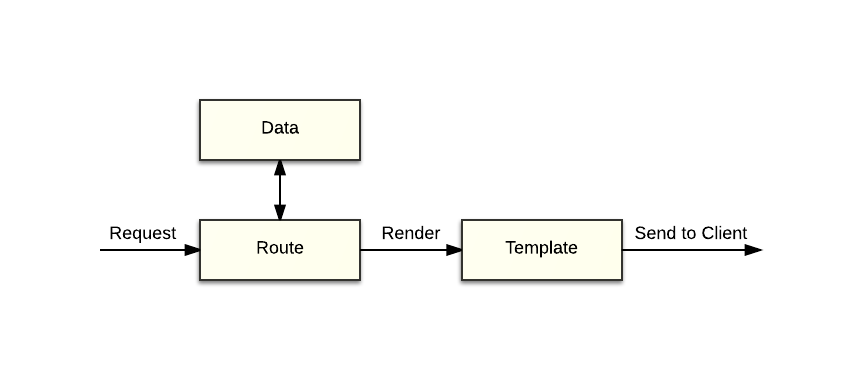
\includegraphics[scale=0.8]{flaskprocess}
		\caption{The Flask request process}
		\label{fig:flaskprocess}
	\end{figure}

	\paragraph{Internal Workings} % title
	% - Communication with storage server{storing remote access_token etc}
	% - GitHub API, login access_token, emails, list of repos for cloning etc
	% - Connecting to MongoDB on storage server

	\paragraph{Routes}

	% Every route
		% Login shit etc
		% Talking to storage for dashboard
		% Game engine, discuss how the template loads all JS, JSON etc

	\subsection{Storage Server}
	% What it is. It's a restful API for accessing files.
	The storage server is where all user created games are stored and retrieved. The storage 
	% each route outputs JSON, even on failure
	% - Why this was it's own server
	The development of a separate server for storing and retrieving files was determined to be necessary to allow for the automatic scaling of the web application

	\paragraph{Architectural Pattern.}
	The software pattern used for the storage server is similar to the MVC system generally used in Flask, however MVC is suited towards applications that have a user interface; a `view'. In this case the JSON output by the RESTful API could be considered the view, with the controller being routes and the model being the file structures.
	% - Pattern - MVC-like
	% - restful API, flask app
		% - GitPython usage
		% - git operations, access_token, remotes
	% - Talk about each API route individually

	% - mongodb
	\subsection{Game Engine}
	% - ECS pattern
	% - "Game" object.
	% - Loading from JSON, initialization
	% - Walkthrough of how the process works. Setting up renderer in Game, updating all scenes with deltatime, updating all entities, updating all components.
	% - Adding, removing components
	% - Using Three.js - setting up the renderer, setting up the Scene to add threeobjs as they are added
	% - Using Ammo.js - Setting up the world, gravity etc, adding ammoobjs as they are added
	% - Simplifying the two libraries into the ECS architecture, predefined components
	% 	This was achieved by etc.
	% - Each pre-defined component
	\subsection{Game Editor}
	% - Pseudo MVC microframework
		% Looked at frameworks, all too heavy
		% Just made my own to keep it simple, based on something similar to backbone
	% - Detail each view
	% - Scene view - 
			% How it loads the gamedata, selection object
	% - Tying in the game engine with the storage backend
	% - Properties of both the gamedata json and the displayed game entities
	% - Scripts, Ace editor
	% - autosaving
	\subsection{Scalable Cloud Deployment}
	% - Setting up AWS
	% - Load balancing, separating web from storage
	% - SSH, Git, tools
	% - Deploying to Elastic Beanstalk {eb cli}
	% - Storage server {Setting up MongoDB, git, cloning the storage repo}
		% - Deployment was difficult compared to Elastic Beanstalk (used git to deploy latest version)

\section{Deployment to AWS}
% How everything was deployed etc

\section{Key Development Components}
% Identify key development components
% Key components were the game engine, editor, web server (load balancing) and storage.
% Git integration wasn't as important to functionality

\section{External APIs}
% Indentification/explanation of external APIs used vs own code. 

\section{List of Classes}
% List of classes of your code
% Write block comments for code during this process?